\documentclass[border=10pt]{standalone}
\usepackage[svgnames]{xcolor}
\usepackage{amsmath}
\usepackage{pgfplots}
\pgfplotsset{compat=newest}
\usepackage[sfdefault]{FiraSans}
\usepackage{FiraMono}
\renewcommand*\familydefault{\sfdefault}
\begin{document}
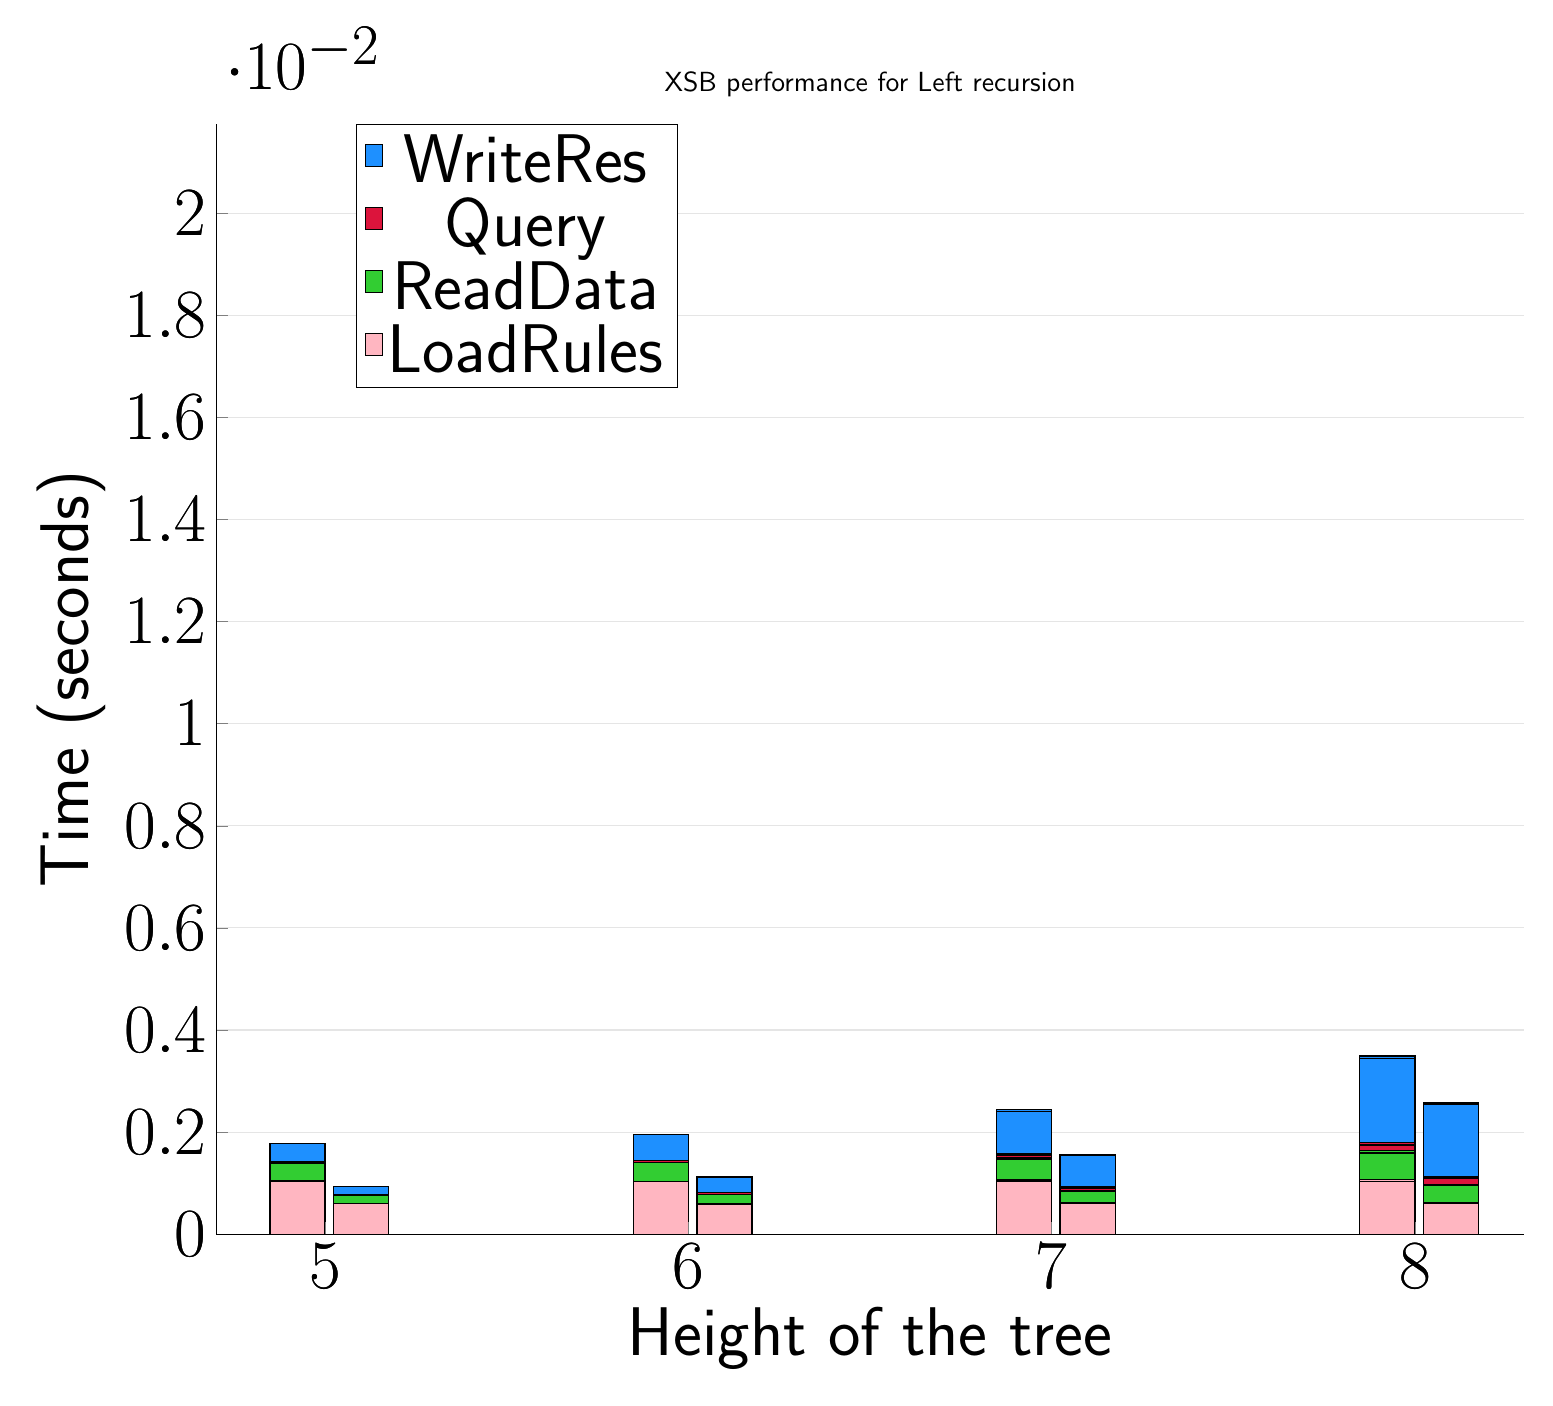
\begin{tikzpicture}
	\begin{axis}[
			ybar stacked,
			title={XSB performance for Left recursion},
			bar shift=-10pt,
			width=1.5\textwidth,
			bar width=0.7cm,
			ymajorgrids, tick align=inside,
			major grid style={draw=gray!20},
			xtick=data,
			ymin=0, ymax=0.02175771713256836,
			axis x line*=bottom,
			axis y line*=left,
			enlarge x limits=0.1,
			legend style={
					at={(0.23, 1)},
					anchor=north,
					legend columns=1,
					font=\Huge,
				},
			ylabel={Time (seconds)},
			xlabel={Height of the tree},
			label style={font=\Huge},
			tick label style={font=\Huge},
		]
		\addlegendimage{fill=DodgerBlue, draw=black, line width=0.2pt}
		\addlegendentry{WriteRes}
		\addlegendimage{fill=Crimson, draw=black, line width=0.2pt}
		\addlegendentry{Query}
		\addlegendimage{fill=LimeGreen, draw=black, line width=0.2pt}
		\addlegendentry{ReadData}
		\addlegendimage{fill=LightPink, draw=black, line width=0.2pt}
		\addlegendentry{LoadRules}
		\addplot +[fill=LightPink, draw=black, line width=0.5pt] coordinates {
				(5, 0.001040649414062499)
				(6, 0.00102710723876953)
				(7, 0.001060175895690918)
				(7, 0.001049900054931641)
				(7, 0.0010412454605102542)
				(8, 0.0010706424713134762)
				(8, 0.001027107238769531)
				(8, 0.001035308837890625)
			};
		\addplot +[fill=LimeGreen, draw=black, line width=0.5pt] coordinates {
				(5, 0.0003555059432983399)
				(6, 0.0003793478012084961)
				(7, 0.000444936752319336)
				(7, 0.00043499469757080067)
				(7, 0.0004253625869750976)
				(8, 0.0005724906921386718)
				(8, 0.0005681514739990233)
				(8, 0.0005465745925903321)
			};
		\addplot +[fill=Crimson, draw=black, line width=0.5pt] coordinates {
				(5, 2.4318695068359392e-05)
				(6, 4.000663757324219e-05)
				(7, 7.38382339477539e-05)
				(7, 7.290840148925782e-05)
				(7, 7.352828979492187e-05)
				(8, 0.00015578269958496088)
				(8, 0.00015473365783691412)
				(8, 0.0001583099365234375)
			};
		\addplot +[fill=DodgerBlue, draw=black, line width=0.5pt] coordinates {
				(5, 0.00036025047302246083)
				(6, 0.0005031824111938477)
				(7, 0.0008610963821411132)
				(7, 0.0008860111236572264)
				(7, 0.0008599519729614256)
				(8, 0.0016905069351196278)
				(8, 0.0016886234283447269)
				(8, 0.0017058610916137686)
			};
	\end{axis}
	\begin{axis}[
			ybar stacked,
			bar shift=13pt,
			width=1.5\textwidth,
			bar width=0.7cm,
			ymajorgrids, tick align=inside,
			major grid style={draw=none},
			xtick=data,
			ymin=0, ymax=0.02175771713256836,
			axis x line*=none,
			axis y line*=none,
			enlarge x limits=0.1,
			label style={font=\Huge},
			tick label style={font=\Huge},
		]
		\addplot +[fill=LightPink, draw=black, line width=0.5pt] coordinates {
				(5, 0.0006008000000000005)
				(6, 0.0005957)
				(7, 0.0006129999999999997)
				(7, 0.0006053000000000005)
				(7, 0.0006018999999999998)
				(8, 0.0006132999999999998)
				(8, 0.0005990999999999998)
				(8, 0.0006050000000000007)
			};
		\addplot +[fill=LimeGreen, draw=black, line width=0.5pt] coordinates {
				(5, 0.0001602999999999997)
				(6, 0.0001879000000000004)
				(7, 0.0002433000000000004)
				(7, 0.00023979999999999978)
				(7, 0.00023679999999999977)
				(8, 0.0003601999999999996)
				(8, 0.00035109999999999964)
				(8, 0.0003507999999999996)
			};
		\addplot +[fill=Crimson, draw=black, line width=0.5pt] coordinates {
				(5, 1.8999999999999916e-05)
				(6, 3.479999999999992e-05)
				(7, 6.669999999999993e-05)
				(7, 6.76000000000003e-05)
				(7, 6.659999999999982e-05)
				(8, 0.00014820000000000002)
				(8, 0.00014599999999999948)
				(8, 0.00014980000000000033)
			};
		\addplot +[fill=DodgerBlue, draw=black, line width=0.5pt] coordinates {
				(5, 0.0001587000000000004)
				(6, 0.0003006000000000001)
				(7, 0.0006444000000000002)
				(7, 0.0006502999999999998)
				(7, 0.0006463999999999996)
				(8, 0.001449)
				(8, 0.0014487000000000002)
				(8, 0.0014464)
			};
	\end{axis}
\end{tikzpicture}

\end{document}
